%DO NOT MESS AROUND WITH THE CODE ON THIS PAGE UNLESS YOU %REALLY KNOW WHAT YOU ARE DOING
 \chapter{Functions of random variables }

\section{Normal distribution and uniform distribution }
\noindent \textbf{Task:} Transform the $N(\mu, \sigma^2)$ distributed random variable \textit{X} into a standard normal distributed random variable. Transform on \textit{[a, b]} uniformly distributed random variable \textit{X} such that it is uniformly distributed on [-1/2,1/2]. 

\noindent \textbf{Solution:}\\
\noindent \textbf{Description}\\
\noindent The standard normal distribution is a special case of the normal distribution. It is the distribution that occurs when a normal random variable has a mean, ($\mu$) of zero and a standard deviation, $(\sigma)$of one. The normal random variable of a standard normal distribution is called a standard score. Every normal random variable \textit{X} can be transformed into a standard normal distribution via the following equation:
$$ Y = \frac{X-\mu}{\sigma}$$
\noindent Where \textit{X} is a normal random variable, $\mu$ is the mean of \textit{X}, and $\sigma$ is the standard deviation of \textit{X.}

\noindent To transform a normal distribution of $ X \sim N(\mu, \sigma)$ into into a standard normal distribution,  $Y \sim N (0,1)$ must be considered. The probability density function of normal distribution can be given as,
$$f_x(x)=\frac{1}{\sqrt{2\pi\sigma^2}}\text{exp}\left\{-\frac{(x-\mu)^2}{2\sigma^2}\right\}, \; \:  x \in R$$ 
\noindent The working of the transformation is possible when, $ y = g(x) =\frac{x-\mu}{\sigma}$.
\noindent When, the mean $(\mu)$ is 0, $y  = g(x = \frac{x}{\sigma})$. Using the inverse property, it can be written as, 
$$ x = g^{-1}(y) = \sigma x+\mu  $$ 
\noindent The probability density function of \textit{Y} can be given as,
$$f_y(y) = \frac{f_x(x)}{|\frac{dF_Y}{dy}|}\:\:   at \:\: x = g^{-1}(y)$$ 
\noindent The probability density function of \textit{X} after inserting $x = g^{-1}(y)$ can be given as,
$$f_x(x) = \frac{\frac{1}{\sqrt{2\pi\sigma^2}}\text{exp}\left\{-\frac{(\sigma y+\mu-\mu)^2}{2\sigma^2}\right\}}{\frac{1}{\sigma}}$$
$$f_x(x)  = \frac{1}{\sqrt{2\pi\sigma^2}}\text{exp}\left\{-\frac{y^2}{2}\right\}, \; \: y \in R$$
\noindent Taking the derivative of the function \textit{g(x)},
$$ \frac{\partial g(x)}{\partial x} = \frac{\partial}{\partial x}(\frac{x}{\sigma} - \frac{\mu}{\sigma})  = \frac{1}{\sigma}  $$
\noindent Substituting this in the probability density function of \textit{Y}, we get
$$f_y(y)  = \frac{1}{\sqrt{2\pi}}\text{exp}\left\{-\frac{y^2}{2}\right\}, \; \: y \in R$$
\noindent This is the transformed form of normal distribution variable to standard normal distribution variable.

\noindent \textbf{Transformation of uniformly distributed random variable}\\
\noindent Consider the random variable  $ X \sim R[a, b]$ which is a rectangular distribution between interval \textit{a} and \textit{b}. The maximum value of this function is $1/(b-a).$ Our aim is to obtain the desired random variable,   $ Y \sim R[-1/2, 1/2]$. In order to achieve this, we create another random variable $ \textit{\~{X}} = X - a.$\\ \\
\noindent The corresponding density function has changed from rectangular function with limits $[a, b]$ to limits $[0, b-a].$ The height of both \textit{X} and \textit{\~{X}} will be the same, i.e, $1/(b-a).$ Extending this further and taking another random variable, $\textit{\^X} = (X - a)/(b - a) =  \textit{\~{X}}/(b - a).$ Thus for this random variable, the graph envelops everything inside the rectangular region 0 and 1, with the maximum value of  $\textit{\~{X}}/(b - a).$ \\ \\
\noindent Now, this random variable will help us in generating our desired random variable,  $Y \sim R[-1/2, 1/2]$
\noindent For our desired variable, we consider 
$$Y = \textit{\^{X}} - (1/2) $$
$$Y = ((X - a) / (b - a)) - 1/2 $$
 \begin{figure}[!ht]
 \centering
 \subfloat[][]{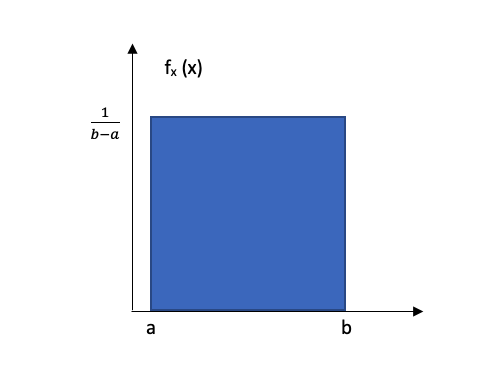
\includegraphics[width=.47\textwidth]{1.png}}\quad
 \subfloat[][]{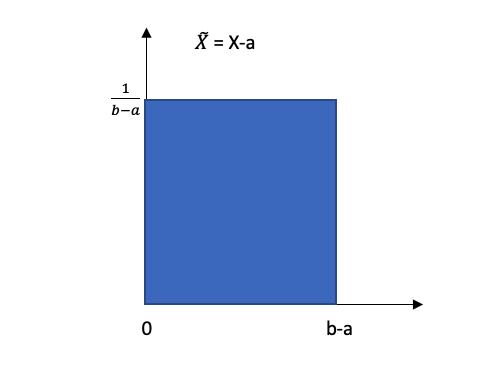
\includegraphics[width=.47\textwidth]{2.png}}\\
 \subfloat[][]{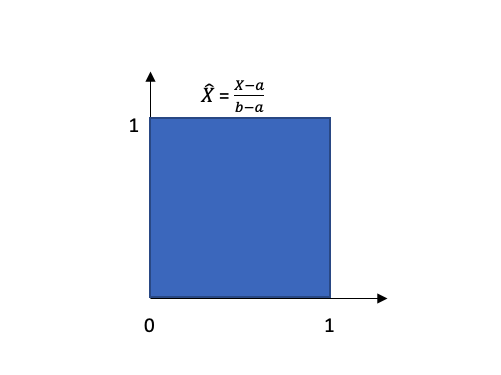
\includegraphics[width=.47\textwidth]{3.png}}\quad
 \subfloat[][]{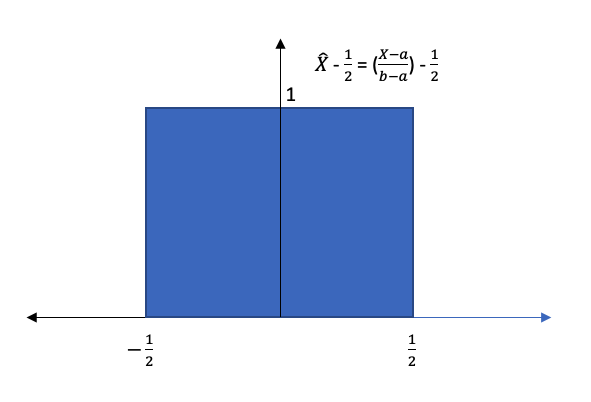
\includegraphics[width=.47\textwidth]{4.png}}
 \caption{Transformation of uniformly distributed random variable}
\end{figure}
\noindent Hence we obtain the desired uniformly distributed random variable, i.e., if \textit{X} is a random variable in [a, b], the \textit{Y} is also a rectangular distribution in $[-1/2, 1/2].$ In practical this type of variable helps us in modelizing the quantization error, which jumps from one point to another over a region.

%%%%%%%%%%%%%%%%%%%%%


\section{Exponential distribution}
\noindent \textbf{Task:} Determine the expected value, the variance and the density function of  $Y = -\frac{1}{a}lnX$ for $a>0,$ when \textit{X} is uniformly distributed on (0, 1). Which other distribution has the same density function, as the exponential distribution for $\alpha = 1/2$ ?

\noindent \textbf{Solution:}\\
\noindent The distribution function $F_Y(y)$ defined by the probability of the random variable, $Y = - \frac{1}{\alpha}\text{ln}(X)$ for $\alpha > 0$ and \textit{X} is uniformly distributed on [0, 1] can be given as,
$$  F_Y(y) = P(Y \leq y)   $$
$$  F_Y(y) = P(\frac{-1}{\alpha}\text{ln}X \leq y) = P(e^{-\alpha y} \leq X)  $$
$$  F_Y(y) =  1 - e^{-\alpha y}$$
\noindent The relationship between the density and the distributed function in the used, i.e.,
$$ f_Y = \frac{\partial F_Y}{\partial y} $$
\noindent Where, $f_y$ is the probability density function and $F_y$ is the distribution function of \textit{Y}. Therefore,
$$ F_Y = [1 - e^{-\alpha y}] . 1_{[0,1]}(y) $$
\noindent The derivative will be,
$$ \frac{\partial F_Y}{\partial y} = \alpha e^{-\alpha y} . 1_{[0,1]}(y) $$
\noindent Now, the probability density function is given as,
$$ f_y(y) = \alpha e^{-\alpha y} $$

\noindent \textbf{The expected value (mean):}\\
$$E(Y) = \int_{-\infty}^{\infty} y f_Y(y) dy $$
\noindent Now substituting for $f_Y{y},$
$$E(Y) = \int_{0}^{\infty} y \alpha e^{-\alpha y}dy$$
$$E(Y) = \alpha\left[\left.-\frac{1}{\alpha}y e^{-\alpha y}\right|_{0}^{\infty}-\int_{0}^{\infty}-\frac{1}{\alpha}e^{-\alpha y}dy\right]$$
$$E(Y)=\left.-\frac{1}{\alpha}e^{-\alpha y}\right|_{0}^{\infty}=\frac{1}{\alpha}$$

\noindent \textbf{The variance :}\\
$${\sigma_Y}^{2} = E(Y-E(Y))^2=E(Y^2)-E(Y)^2$$
\noindent $ E(Y^2) $ can be calculated as,
$$E(Y^2) = \int_{-\infty}^{\infty}y^2 f_y(Y) dy = \int_{0}^{\infty}y^2 \alpha e^{-\alpha y}dy $$
$$E(Y^2) = \alpha\left[\left.-\frac{1}{\alpha}y e^{-\alpha y}\right|_{0}^{\infty}-\int_{0}^{\infty}-\frac{2}{\alpha}ye^{-\alpha y} dy\right]$$
$$E(Y^2) = 2\int_{0}^{\infty}y e^{-\alpha y} dy = \frac{2}{\alpha^2}$$
$${\sigma_Y}^{2} = \frac{2}{\alpha^2}-\frac{1}{\alpha^2}=\frac{1}{\alpha^2}$$

\noindent \textbf{The other distribution function:}\\
\noindent If we Suppose $X \sim X_n^2$ then the density function is given as 
$$f_X(x)=\frac{1}{2^{\frac{n}{2}}\Gamma(\frac{n}{2})}.x^{\frac{n}{2}-1}e^{-\frac{x}{2}}$$
\noindent When $n = 2$,
$$\Gamma(1)= 1 $$
$$f_X(x) = \frac{1}{2} e^{\frac{-x}{2}}$$
\noindent The value of density function $f_Y(y)$ when $\alpha = 1/2$ is given as,
$$f_y(y) = \frac{1}{2}  e^{\frac{-y}{2}} $$
\noindent Comparing $f_X(x)$ and $f_Y(y)$, we conclude that the other distribution function having the same density function as the exponential function is $X_2^2 $ distribution.\\
 
%%%%%%%%%%%%%%%%%%% 
 
\section{Sum of Random Variables}
\noindent \textbf{Task:} Determine the expected value, the variance and the density function of  $Z=X+Y,$ when \textit{X} and \textit{Y} are two stochastically independent, on [0,1] uniformly distributed random variables.\\

\noindent \textbf{Solution:} \\
\noindent \textbf{Description:} 
\begin{figure}[H]
\centering
{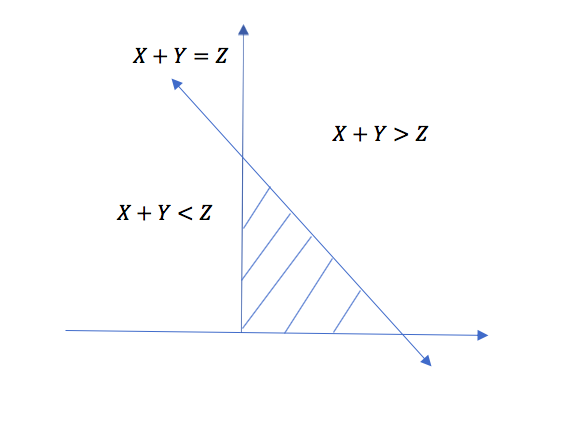
\includegraphics[scale=0.48]{5.png}}
\caption{function $X + Y = Z$}
\end{figure}

\noindent Let \textit{X} and \textit{Y} be two independent random variables distributed on the interval [0, 1] that is, $X, Y \sim R(0,1)$ and $Z = g(X, Y) = X+Y$. The distribution function for the random variable \textit{Z} can be expressed as,
$$F_Z(z) = P(Z \leq z) = P(X+Y \leq z) = \int_{-\infty}^{\infty}\int_{\infty}^{z-x} f_{XY}\text{(xy) dx dy}$$\\
\noindent The density function of the random variable \textit{Z} is the derivative pf the distribution function,
$$f_Z(z)=\frac{\partial F_Z(z)}{\partial z}$$\\
\noindent Substituting $F_Z(z)$ in $f_Z(z)$,
$$f_Z(z) = \frac{\partial}{\partial z}\int_{-\infty}^{\infty}\int_{-\infty}^{z-x}f_{XY}\text{(x,y) dy dx}$$\\
$$f_Z(z) = \int_{-\infty}^{\infty}\frac{\partial}{\partial z}\left(f_{XY}(\text{x, z-x}) - f_{XY}(\text{x},-\infty)\right)\text{dx}$$
$$f_Z(z) =\int_{-\infty}^{\infty}f_{XY}(\text{x, z-x) dx}$$
\noindent If we assume \textit{X} and \textit{Y} as two independent random variables, then we get the density function for sum of two random variables as,
$$f_Z(z) =\int_{-\infty}^{\infty}f_X(\text{x}) f_Y(\text{z - x}) \text{dx} $$ 
\noindent This is a convolution integral and it represents the sum of two random variables.
$$f_Z(z) = \int_{-\infty}^{\infty}1_{[0,1]}\text{(z-x) dx} = \int_0^1 1_{[0,1]}\text{(z-x) dx}$$\\
\noindent Consider $ u = z - x $, $\Rightarrow$ $ dx = -du $
$$f_Z(z) = -\int_z^{z-1}1_{[0,1]}\text{(u) du} = \int_{z-1}^{z}1_{[0,1]}\text{(u) du}$$ 
\noindent The function $1_{[0,1]}\text{(u)}$ is always zero expect when $0 \leq \text{u} \leq 1$ And, we can discuss the following cases:\\
\textbf{Case 1:   z$<$0 and z$>$2:}
$$f_Z(z)= \int_{z-1}^z 1_{[0,1]}\text{(u) du}$$
$$f_Z(z) = 0$$

\textbf{Case 2: 0 $\leq$ z $\leq$ 1:}
$$f_Z(z) = \int_{z-1}^z 1_{[0,1]}\text{(u) du} = \int_{z-1}^0 1_{[0,1]}\text{(u) du} + \int_0^z 1_{[0,1]}\text{(u) du} = \left .u\right|_0^z$$
$$f_Z(z) = z$$

\textbf{Case 3: 1 $<$ z $\leq$ 2:}
$$f_Z(z) = \int_{z-1}^1 1_{[0,1]}\text{(u) du} = \left.u\right|_{z-1}^1 =1 - z +1 $$
$$f_Z(z) = 2 - z$$

The resulting density function can be expressed as:
\[ f_z(z)=
	\begin{cases}
		\text{0,} &\quad\text{otherwise}\\
		\text{z,} &\quad\text{$0 \leq z \leq 1$}\\
		\text{2 - z,} &\quad\text{$1 \leq z \leq 2$}\\	
		\end{cases}
\]\\
\noindent \textbf{The expected value (mean):}
$$ E(Z) = \int_{-\infty}^{\infty} z f_Z(z) dz = \int_0^1 z^2 dz + \int_1^2z(2-z) dz $$
$$ E(Z) = \left.\frac{z^3}{3}\right|_0^1+\int_1^22zdz - \int_1^2 z^2 dz$$
$$ E(Z) = \frac{1}{3} + \left. z^2 \right|_1^2 - \left.\frac{z^3}{3}\right|_1^2 = \frac{1}{3} + 3- \frac{7}{3}$$
$$E(Z) = 1$$
\noindent For two independent random variables, E(Z) = E(X+Y) = E(X) + E(Y) and for uniformly distributed  random variable on the interval [0,1], E(X) = E(Y) = $\frac{1}{2}$, hence E(Z) = $\frac{1}{2} + \frac{1}{2} = 1 $.

\noindent \textbf{The variance :}
$${\sigma_Z}^{2} = E(Z-1)^2 = \int_{-\infty}^{\infty}(Z-1)f_z(z) dz$$
We have Z=X+Y,
$${\sigma_Z}^{2} =E(Z-1)^2 = E(X+Y-1)^2 = E\left(\left(X-\frac{1}{2}\right)+\left(Y-\frac{1}{2}\right)\right)^2$$
$${\sigma_Z}^{2} = E(X+Y-1)^2 = E\left(\left(X-\frac{1}{2}\right)^2+2\left(X-\frac{1}{2}\right)\left(Y-\frac{1}{2}\right)+\left(Y-\frac{1}{2}\right)^2\right)$$
\noindent We know that, Cov(X,Y) = 0. Because X and Y are independent.
$${\sigma_Z}^{2} = \frac{1}{12} + \frac{1}{12} $$
$${\sigma_Z}^{2}=\frac{1}{6}$$

%%%%%%%%%%%%%%%%%%%

\section{Product of random variables}
\noindent \textbf{Task:} Calculate the expected value, the variance and the density function of $Z = XY,$ when \textit{X} and \textit{Y} are two stochastically independent, on [0, 1] uniformly distributed random variables.\\

\noindent \textbf{Solution:} 
\noindent Let $Z = XY$ be the product of two random variables \textit{X} and \textit{Y}, where \textit{X} and \textit{Y} are identical, independent and uniformly distributed random variables, i.e., $X, Y \sim R[0, 1]$ \\
\noindent In order to get the density function of the product of the two random variables, we introduce an auxiliary variable, $W = Y.$ We also consider that the density of the bivariate function $f(x, y)$ is known. Therefore, \textit{Y} is a function of $h(x, y)$,
$$ x = \frac{z}{y} = \frac{z}{w} = g^{-1}(z, w)  $$
$$ y = w = h^{-1}(z, w)  $$
\noindent To determine the distribution of the transformed random variables, the Jacobian matrix is emplyed,
\[J(x, y) =
\begin{bmatrix}
\frac{\partial g}{\partial x}  & \frac{\partial g}{\partial y}\\
\frac{\partial h}{\partial x}  &  \frac{\partial h}{\partial y}\\
\end{bmatrix}
=
\begin{bmatrix}
y & x\\
0 & 1\\ 
\end{bmatrix}
\]
$$|\text{det}(J(x, y))| = |y| = |w| $$
\noindent The bivariate density function is given by,
$$ f_{Z,W}(z,w) = \frac{f_{XY}(g^{-1}(z, w), h^{-1}(z, w))}{|\text{det} (J)|}     $$
$$ f_{Z,W}(z,w) = \frac{f_{XY}(z/w, w)}{|w|}     $$
\noindent As the variable \textit{X} and \text{Y} are independent, the probability function can be written as,
$$ f_{XY} = f_X \bigg(\frac{z}{w}\bigg) f_Y(w)  $$
\noindent The probability density function of \textit{Z} is given by,
$$f_Z(z) = \int_{-\infty}^{\infty}f_{ZW}(z, w)dw$$
$$f_Z(z) = \int_{-\infty}^{\infty}\frac{f_{X, Y}(\frac{z}{w}, w)}{|w|} dw $$
$$f_Z(z) = \int_{-\infty}^{\infty}\frac{f_X(\frac{z}{w})f_y(w)}{|w|}dw $$
$$ f_Z(z)  = \int_0^1 \frac{f_X(\frac{z}{w})}{|w|}dw$$

\textbf{Case 1:   z$<$0 i.e.,  $\frac{\textbf{z}}{\textbf{w}}$$<$0:}
$$ f_Z(z)  = 0$$

\textbf{Case 2: 0 $<$ z $\leq$ 1, i.e,  z $\leq$ w $<$ 1 :}
\noindent This means,  0 $<$ $\frac{z}{w}$ $\leq$ 1
$$  f_Z(z) = \int_z^1 \frac{1}{w} dw = \left.\text{ln}(w)\right|_z^1 $$
$$  f_Z(z) = -\text{ln}(z)$$

\textbf{Case 3:   z$>$1 i.e.,  $\frac{\textbf{z}}{\textbf{w}}$$>$1:}
$$ f_Z(z)  = 0$$

\noindent Then, the density function can be expressed by,
\[f_z(z)=
	\begin{cases}
	\text{0}   &\quad\text{$z<0$}\\
	\text{-ln(z)} &\quad\text{0 $\leq z \leq $1}\\
	\text{0}   &\quad\text{$z>1$}\\
	\end{cases}
\]
\noindent \textbf{The expected value (mean):}
$$ E[Z] =  E[XY] = E[X].E[Y] $$
$$E(Z) = \int_{-\infty}^{\infty}zf_Z(z) dz = -\int_0^1z \text{ln}(z) dz = -\left(\left.\frac{z^2}{2}ln (z)\right|_0^1 - \int_0^1\frac{z^2}{2}\frac{1}{z}dz\right) = \left.\frac{z^2}{4}\right|_0^1$$
$$E(Z) = \frac{1}{4}$$

\noindent \textbf{The variance :}
$${\sigma_Z}^{2} = E[Z ^2] - (E[Z])^2 $$
\noindent So, 
$$ E[Z ^2] =  \int_{-\infty}^{\infty}z^2 f_Z(z) dz =  -\int_0^1z^2 \text{ln}(z) dz = \left.\frac{z^3}{9}\right|_0^1 = \frac{1}{9} $$
$$(E[Z])^2 = \frac{1}{16}$$
\noindent Hence, the variance is,
$${\sigma_Z}^{2} = \frac{1}{9} - \frac{1}{16}= \frac{7}{144}$$
%%%%%%%%%%%%%%%%

\section{$\chi^2$ distribution}
\noindent \textbf{Task:} Determine the expected value, the variance and the density of \\
$$Z = \sum\limits_{i=1}^{4} X_i^2$$
where $X_i$(i =1,2,3,4) are four stochastically independent, standard normally distributed random variables. How could one create a random variable from two stochastically independent exponentially distributed random variables that possess the same distribution as \textit{Z}? Calculate the density of \textit{Z} through convolution of the density of an exponential distribution.\\

\noindent \textbf{Solution:} 
\noindent $\chi^2$ distribution defines a property such that its mean coincides with the number of degrees of freedom, \textit{n}. It is mathematically defined as,
$$ Z = \sum_{i=1}^{n} X_i^{2}    $$ 
\noindent Where, $X_i$ is a standard normally distributed random variable. Here, $n = 4$, therefore, the mean is 4 for  $\chi_4^{2} $ distribution. 
\noindent The variance of the distribution is nothing but, twice the degree of freedom. Hence, the variance is 8 for $\chi_4^{2} $ distribution.\\
\noindent \textbf{The expected value (mean):}
\noindent Conventionally, it can also be calculated by,
$$E[Z] = \int_{-\infty}^{\infty} z f_Z(z) dz = \int_0^1 z\Bigg(\frac{1}{4}.z.e^{-\frac{z}{2}}\Bigg)dz $$
  $$E[Z] = 4 $$


\noindent \textbf{The variance:}
\noindent Conventionally, it can also be calculated by,
$${\sigma_Z}^{2} = E[Z ^2] - (E[Z])^2 $$
$${\sigma_Z}^{2} = \int_{-\infty}^{\infty} z^2 f_Z(z)dz -16 $$
$${\sigma_Z}^{2} = 8 $$

\noindent \textbf{Generating a random variable from two exponential distractions:}
\noindent Let us suppose we have two exponentially distributed random variables $X_1$ and $X_2$. Hence we can calculate the density of the sum of $X_1$ and $X_2$ by generating a third random variable \textit{Z}. If $X_i$, $(i = 1, 2, 3,...,n)$n are stochastically independent exponentially distributed random variables with rate parameter, $\alpha$ and mean, $1/\alpha$, then the probability density function is,
$$ f_Z(x) = f_{X_1 + X_2 + ... + X_n}(x) = \alpha e^{-\alpha x} \frac{(\alpha x)^{n-1}}{(n-1)!}      $$
\noindent Thus for $n = 2,$
$$ f_Z(x) = f_{X_1 + X_2 }(x) = \alpha e^{-\alpha x} \frac{(\alpha x)^{2-1}}{(2-1)!} = \alpha^2 x e^{-\alpha x}      $$
\noindent If $\alpha = 1/2$,
\[ f_Z(x) = \frac{1}{4}x e^{-\frac{1}{2}x} \tag{1} \]
\noindent Let us consider a random variable \textit{Z}, which represents a function of a standard normally distributed random variables, such that\\
$$ Z = \sum \limits_{i=1}^{4} X_i^2 $$
\noindent Its probability density function is given by, \\
$ f_Z(x) = \frac{1}{2^n / 2 \Gamma (n/2)} Z^{\frac{n}{2} - 1} e^{-z/2} ,$ \: \: z $>$ 0
\[ f_Z(z) = \frac{1}{4} z e^{-\frac{1}{2}z}   \tag{2} \]

\noindent From equation (1) and equation (2), we conclude that the density of random variable \textit{Z} as a sum of two exponentially distributed random variables is the same as that of$\chi^2$ distributed random variable \textit{Z} with four degrees of freedom, if $\alpha = 1/2$.


\noindent \textbf{Probability Density as convolution of density of exponential random variables:}
\noindent We have four stochastically independent, standard normally distributed random variables, $X_i$ where $(i = 1, 2, 3, 4)$. When these random variables are squared and grouped such that we have two exponentially distributed random variables \textit{X} and \textit{Y} where,\\
$ X = X_1^2 + X_2^2 $ and $ Y = Y_3^2 + Y_4^2 $ \\
\noindent Therefore, the density function for the random variables can be expressed as,
$$ f_X(x) =  \frac{1}{2} e^{-\frac{x}{2}}$$
\noindent and
$$ f_Y(y) =  \frac{1}{2} e^{-\frac{y}{2}}$$
\noindent Now, if we assume that \textit{X} and \textit{Y} generate a new random variable \textit{Z}, such that $Z = X + Y$. Then the bivariate density function for \textit{X} and \textit{Y} gives the probability distribution function of  \textit{Z}.
$$f _Z(z) = \int_{-\infty}^{\infty} f_{(X, Y)}(x, y) \textit{dx}  \textit{dy} = \int_{-\infty}^{\infty} f_{X}(x)  f_{Y}(y) \textit{dx}  \textit{dy}$$
\noindent Substituting $Y = Z - X$,
$$f_Z(z) = \int_0^z f_X(x)f_Y(z - x) dx $$
$$f_Z(z) =  \frac{1}{4}. z. e^{-\frac{z}{2}}$$




 %%%%%%%%%%%%%%%%%

\section{Normal distribution from uniform distribution}
\noindent \textbf{Task:} Calculate the bivariate density $f_{Y_1Y_2}(y_1,y_2)$ of \\
 $Y_1 = \sqrt{-2\text{ln} X_1}\text{sin}(2\pi X_2) $ and each on [0,1] uniformly distributed random variables.\\
\noindent \textbf{Solution:} 
\noindent Given two random variables $X_1$ and $X_2$ which are independent,  identical and uniformly distributed on the interval [0,1] that is $X_1 \sim R(0,1), Y_1 \sim R(0,1)$. The task is to generate bivariate density function of two random variables $Y_1$ and $Y_2$ where,
$$Y_1 = \sqrt{-2\text{ln}(X_1)}sin(2\pi X_2) = g_1(X1,X2)$$
$$Y_2 = \sqrt{-2\text{ln}(X_1)}cos(2\pi X_2) = g_2(X1,X2)$$
\noindent First step is relating $Y_1$ and $Y_2$ with $X_1$ and $X_2$ as follows:\\
$$ Y_1^2 + Y_2^2 = -2\text{ln}(X_1) $$
$$x_1 = g_1^{-1}(y_1, y_2) = \text{exp}\Bigg(-\frac{y_1^2 + y_2^2}{2}\Bigg)$$
$$x_2 = g_2^{-1}(y_1, y_2) = \frac{1}{2 \pi}\text{arctan}{\frac{y_1}{y_2}}$$
\noindent To calculate the bivariate density function,\\
$$f_{Y_1Y_2}(y_1y_2) = \left.\frac{f_{x_1x_2}(x_1, x_2)}{|\text{det}(J)|}\right|_{x_1=g_1^{-1}(y_1, y_2),  \; \: x_2 = g_2^{-1}(y_1, y_2)}$$
\[ f_{Y_1Y_2}(y_1y_2) = f_{x_1x_2}(x_1, x_2) / \frac{\partial (x_1, x_2)}{\partial (y_1, y_2)}  \tag{3} \]
\noindent where,
$$ \frac{\partial (x_1, x_2)}{\partial (y_1, y_2)} = |\text{det} J| $$
\noindent Also, $f_{X_1X_2}(x_1x_2) = f_{X_1}(x_1) f_{Y_1}(y_1)$

\noindent To determine the determinant of the Jacobian Matrix, $J$,
\[J =
\begin{bmatrix}
\frac{\partial g_1(x_1,x_2)}{\partial x_1}  & \frac{\partial g_1(x_1,x_2)}{\partial x_2}\\
\frac{\partial g_2(x_1,x_2)}{\partial x_1}  &  \frac{\partial g_2(x_1,x_2)}{\partial x_2}\\
\end{bmatrix}
=
\begin{bmatrix}
\frac{sin(2\pi x_2)}{x_1\sqrt{-2\text{ln} x_1}}  & 2\pi\sqrt{-2\text{ln} x_1}cos(2\pi x_2)\\
\frac{cos(2\pi x_2)}{x_1\sqrt{-2\text{ln} x_1}}  &  -2\pi\sqrt{-2\text{ln} x_1}sin(2\pi x_2)\\
\end{bmatrix}
\]
$$ |\text{det}(J)| = |\frac{2\pi}{x_1}|$$
\[ |\text{det}(J)| = \frac{2 \pi}{ \text{exp}\Bigg(-\frac{y_1^2 + y_2^2}{2}\Bigg)}   \tag{4} \]

\noindent The joint probability density function of $X_1$ and $X_2$ will be:\\
\[ f_{X_1X_2}(x_1x_2) =
	\begin{cases}
	\text{1}   &\quad\text{0 $\leq x_1, x_2 \leq $1}\\
	\text{0} &\quad\text{otherwise}\\
	\end{cases} \tag{5}
\]
\noindent Now, substituting equation (4) and equation (5) in equation (3), we get,
$$f_{x_1x_2}(x_1x_2) = \frac{1}{2\pi}exp(-\frac{y_1^2+y_2^2}{2})$$

\noindent Bivariate density function can be written as a product of two functions as shown below:\\
$$f_{y_1y_2}(y_1y_2) = \frac{1}{2\pi}\text{exp}(-\frac{y_1^2}{2}).\frac{1}{2\pi}exp(-\frac{y_2^2}{2})=f_{y_1}(y_1).f_{y_2}(y_2)$$
$$f_{y_1}(y1)=\frac{1}{2 \pi}\text{exp}(-\frac{y_1^2}{2})$$
$$f_{y_2}(y2)=\frac{1}{2 \pi}\text{exp}(-\frac{y_2^2}{2})$$
\noindent Each of these two functions represents a density function of a standard uniformly distributed random variable that is $Y_1 \sim N(0,1)$ and $Y_2 \sim N(0,1)$. Thus $Y_1$ and $Y_2$ can be termed now as independent and Standard Normally Distributed Random Variables.


